\documentclass[]{article}
\usepackage{amsmath}
\usepackage{amssymb}
\usepackage{graphicx}
\usepackage[utf8]{inputenc} 
\usepackage{hyperref} 
%opening
\title{}
\author{}

\begin{document}

%\maketitle




%\begin{figure}[H]
%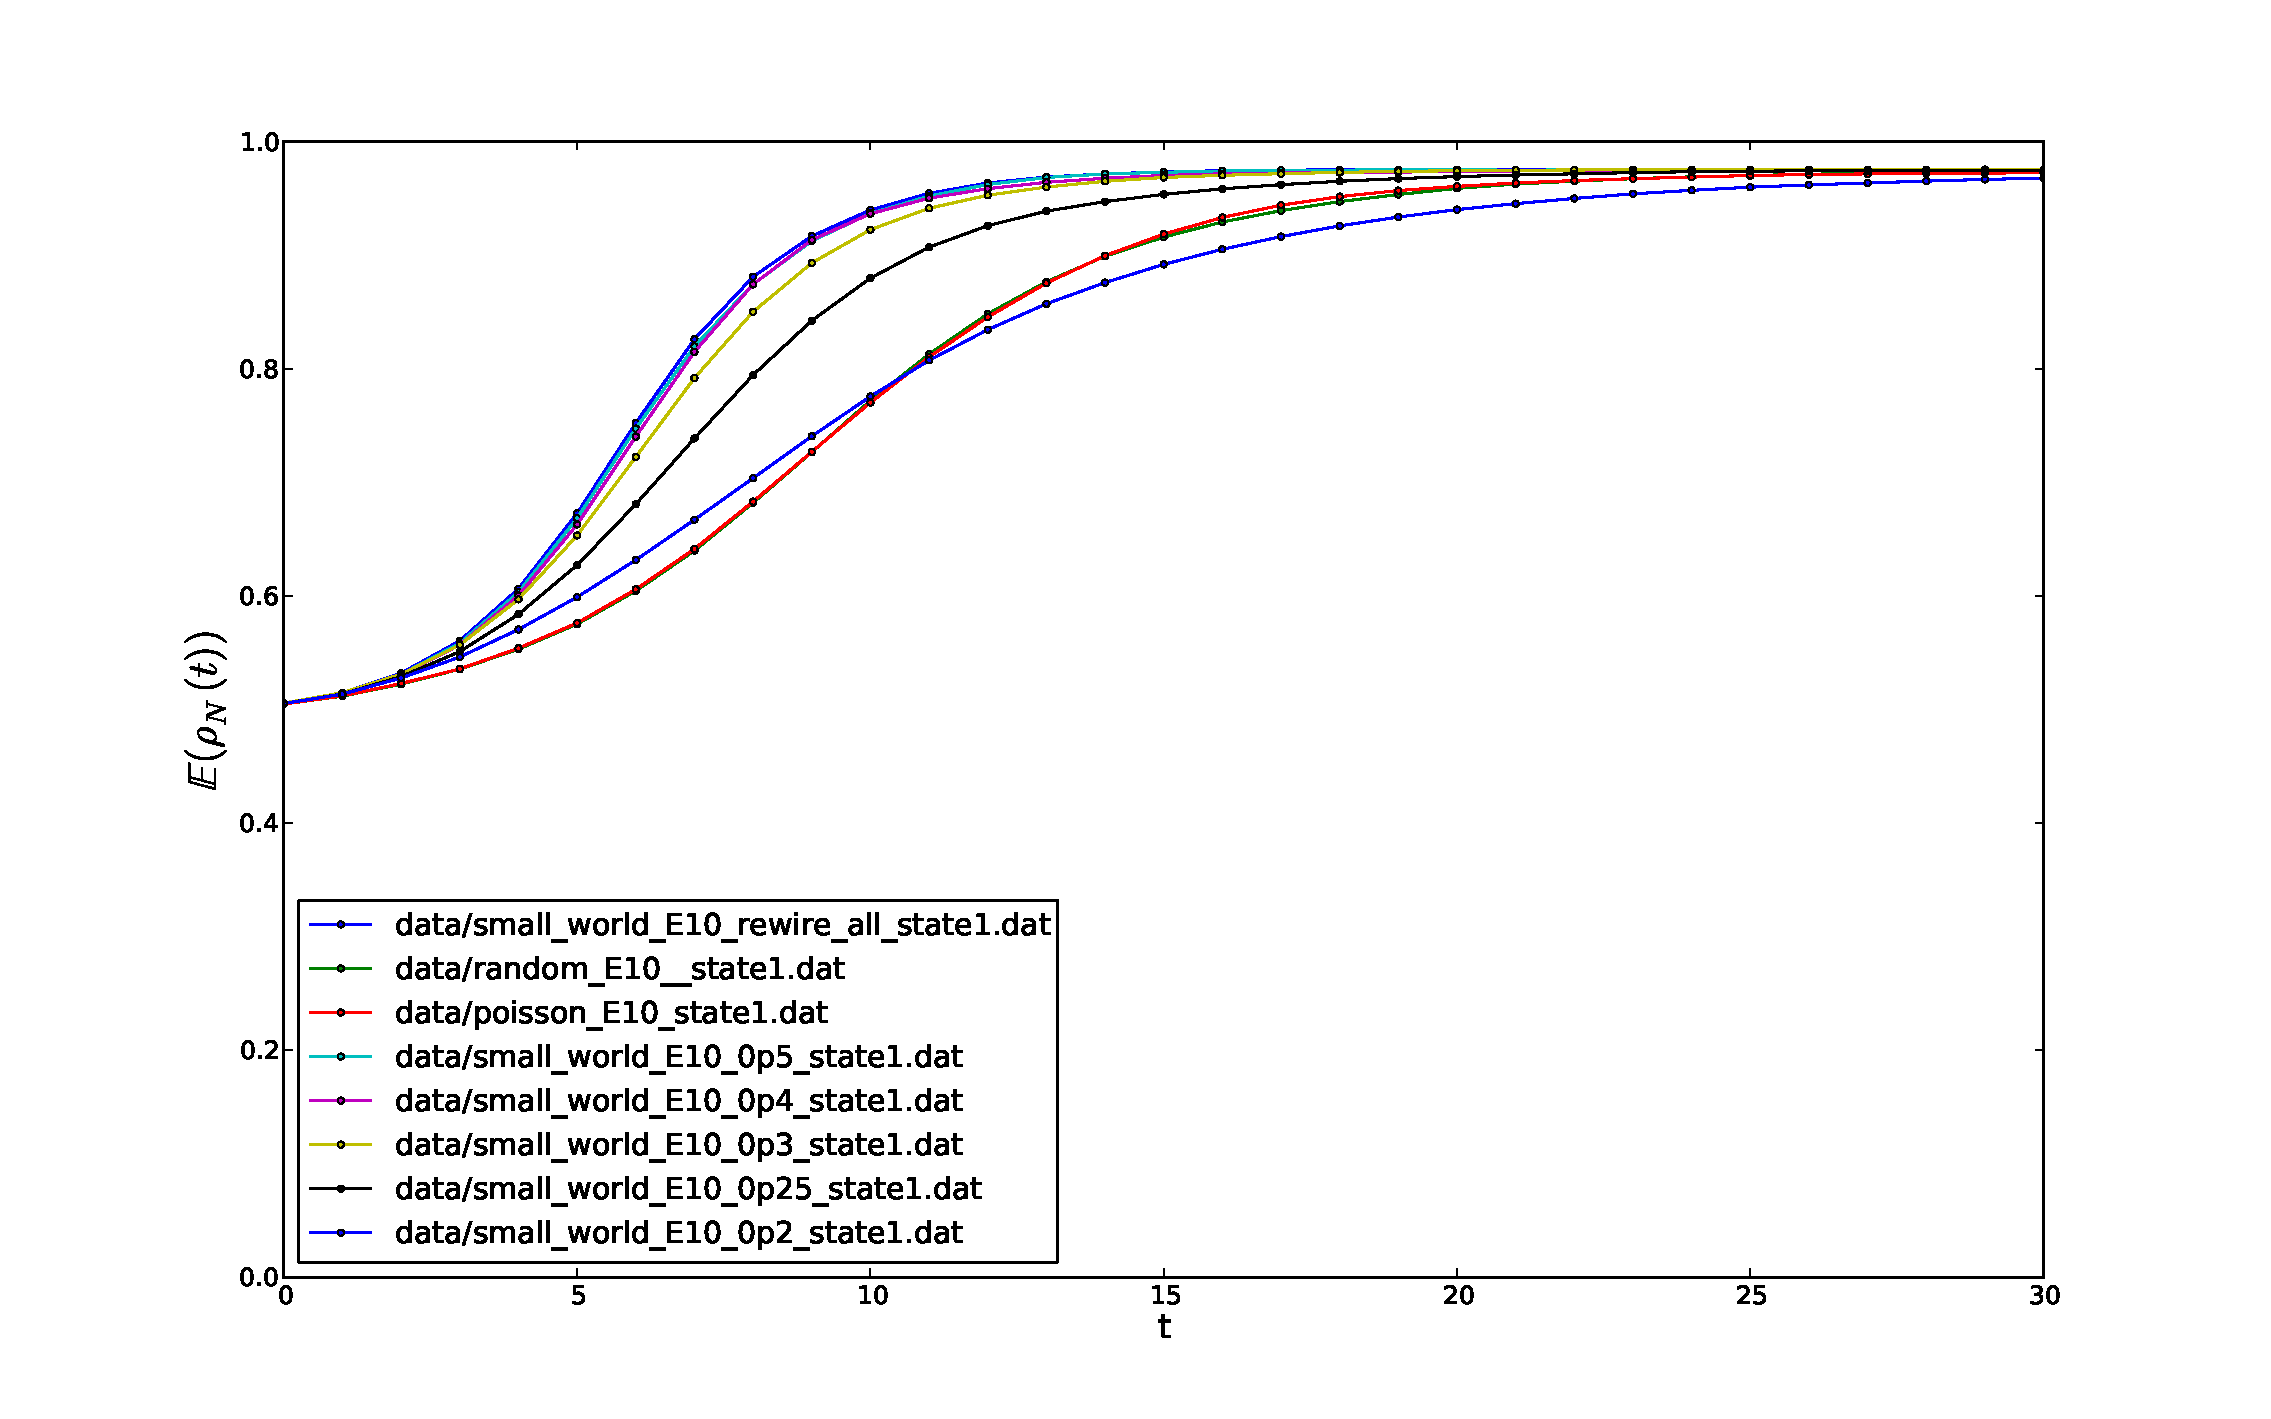
\includegraphics[width=1.1\textwidth]{time_evolution_rewiring_probability_dependency.pdf}
%\caption{Average time evolution of coarse states in small world networks generated with $\beta=0.2, 0.25, 0.3, 0.4, 0.5, 1$ compared to average time evolution in  network with poisson-distributed degrees.}
%\label{fig:time_evolution_beta}
%\end{figure}



%\begin{abstract}
%\end{abstract}
\section{Time evolution of coarse states on static interaction networks with different topologies}
\subsection{Fully connected network}

Figure \ref{fig:time_evolution} shows the ensemble average over 1000 realizations of the average state in a fully connected network as a function of time. Simulations are performed for two different coupling constants $\mathcal{N}(\bar{\nu}=0.5)$ and  $\mathcal{N}(\bar{\nu}=0.05)$ and two different initial conditions $ \mu_{0 n} \sim \mathcal{B} ( \mu; 0.5) $ respectively $ \mu_{0n} \sim\mathcal{B} ( \mu; 0.9 ) $ for $n=1,...,4000$.     %\ref{} . 
 The values of the microscopic parameters are chosen in correspondence with these in the AHS-lattice-model \cite{avitabile14}. Each agent is interacting with all other agents. For small values of the average coupling constant $\bar{\nu}$, the mixed state is the unique macroscopic stable equilibrium.  If the average value of the coupling constant $\bar{\nu}$ is increased, two new macroscopic states arise, suggesting the presence of a pitchfork bifurcation. 

%For a network with 8000 nodes with all-to-all-coupling (all agents in the network interact with all the other agents).
\subsection{Erd\H{o}s-Rényi network}

Above described experiments are repeated with the same simulation parameters and system size, but with all agents randomly connected with on average 100 other agents. The connections don't change in time and the agents only interact with agents they are connected with. Figure \ref{fig:time_evolution_erdos} shows that it took at least 20 iterations to achieve the locked-in states, which is longer than the time needed to reach equilibrium in a fully connected network. For the mixed state however, the relaxation time does not differ significantly between both models.

%\subsection{Small world network}

%The simulations are repeated for a small world network, generated by the Watts-Strogatz-algorithm with rewiring probabilty $\beta$. This accounts for higher clustering in comparison with  Erd\H{o}s-Rényi-networks but for a smaller average path length in comparison with a lattice network  \cite{watts98}. Each agent is connected with on average $K=100$ other agents. (The Watts-Strogatz-alogorithm requires that $N >> K >> \ln(N) >> 1$ where $ K >> \ln(N)$ requires that a random graph whil be connected. ) 
%
% Figure \ref{fig:time_evolution_watts} shows the time evolution on a network with $\beta=0.5$, figure \ref{fig:time_evolution_watts0p1} for a network generated with $\beta=0.1$ (over a longer time period). 
% 
% 
 

%\subsection{Ring lattice}
%
%The simulations are repeated on a ring lattice, with each node connected to its 10 nearest neighbours. Figure \ref{fig:time_evolution_ring} shows that... %the time to achieve the locked-in-states lies between the time on a fully-connected-network and the time on an Erd\H{o}s-Rényi-network with same system size. 
%Figure \ref{fig:time_evolution_ring_long} shows simulation over a longer time period.

\begin{figure}


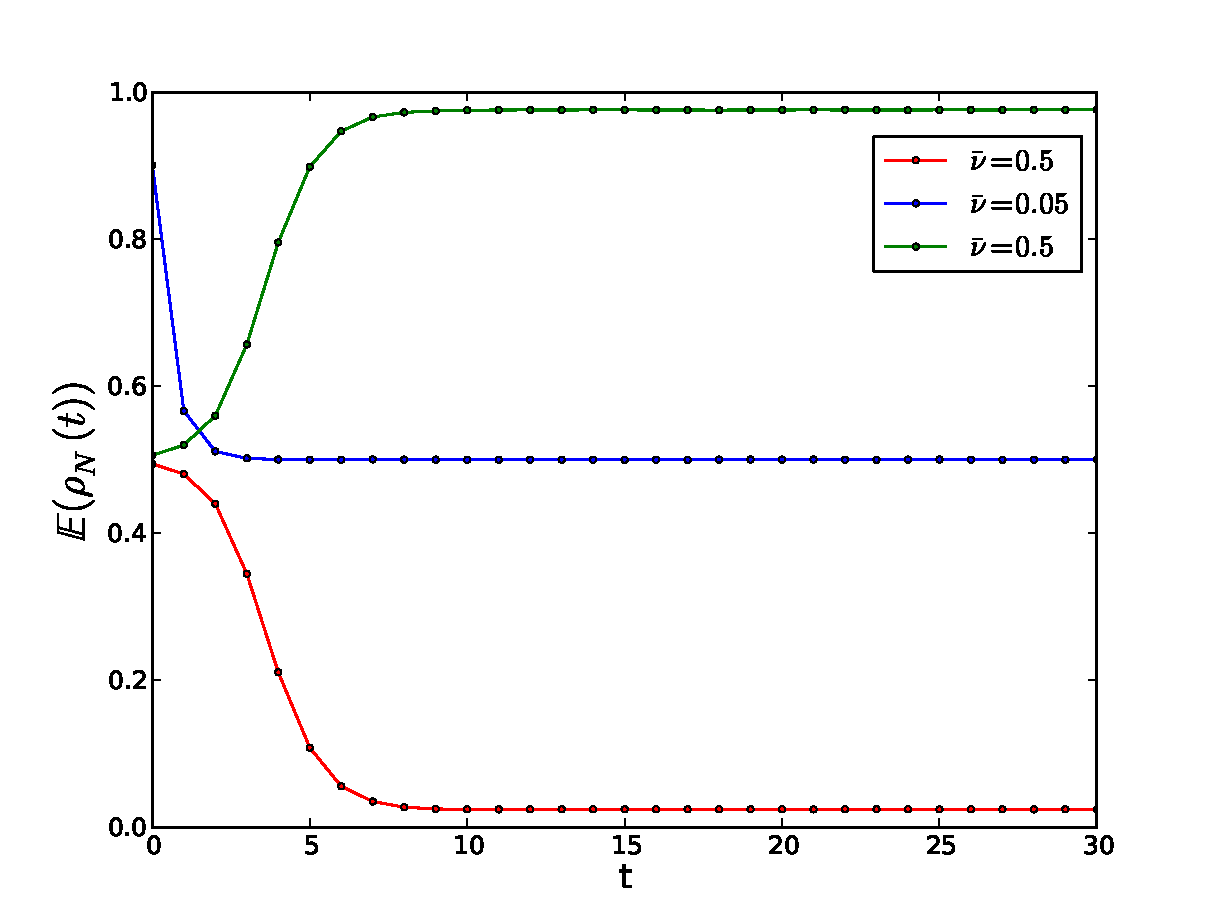
\includegraphics[width=0.9\textwidth]{time_evolution_fully_M1000_N4000.pdf}
\caption{Average time evolution of coarse states in a fully-connected network with 4000 nodes.}
\label{fig:time_evolution}
\end{figure}


\begin{figure}
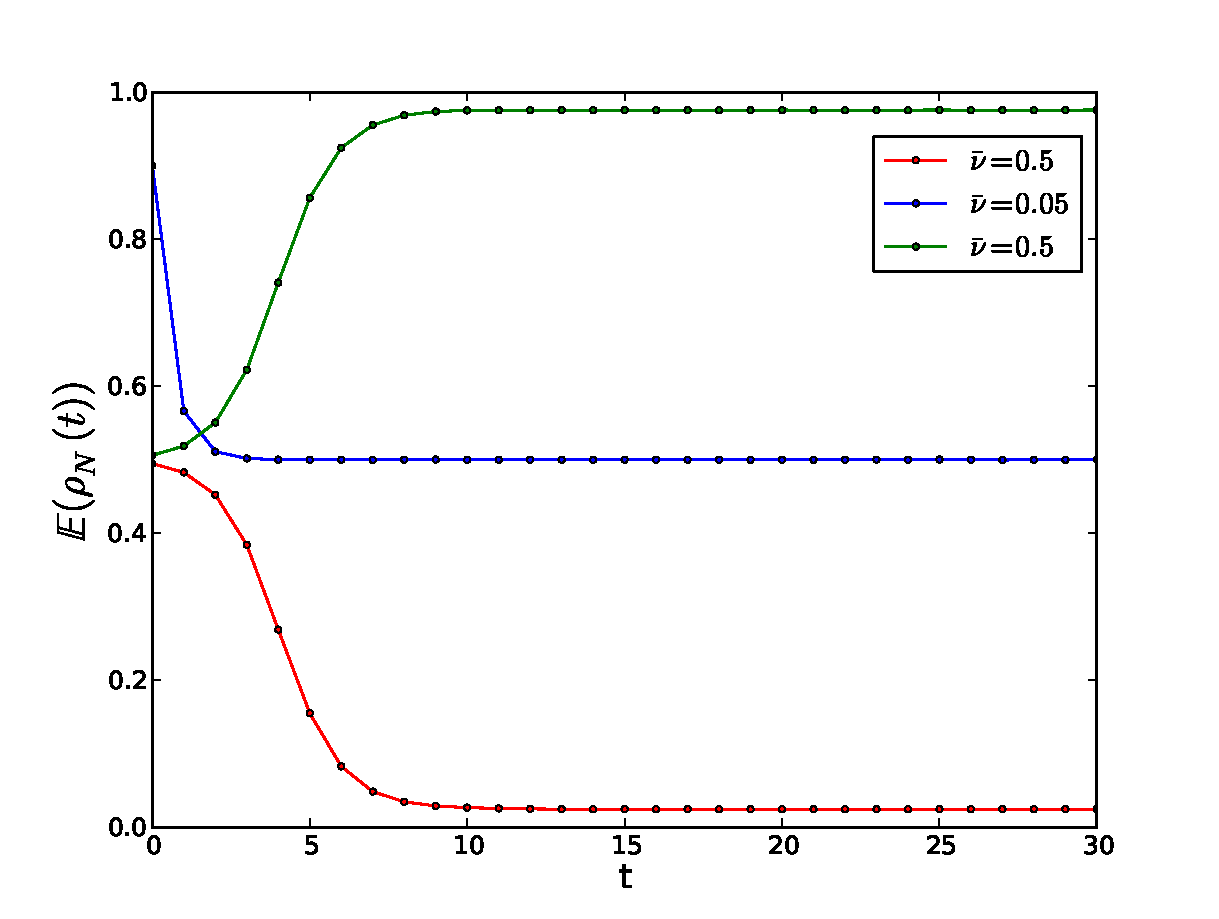
\includegraphics[width=0.9\textwidth]{time_evolution_random_M1000_N4000.pdf}
\caption{Average time evolution of coarse states in an Erd\H{o}s-Rényi network of 4000 nodes with average degree 100.}
\label{fig:time_evolution_erdos}
\end{figure}


\section{Variance of asymptotic equilibria}

The expectation value $\mathbb{E}(\rho_N)$ and the variance $\texttt{var}(\rho_N(t))$ are monitored as a function of time for a collection of different means of the initial states. In Figure \ref{fig:variance_mean} the several orbits on the $(\mathbb{E}(\rho_N),\texttt{var}(\rho_N(t)))$-plane are shown for high values of the interaction strength.  


\begin{figure}
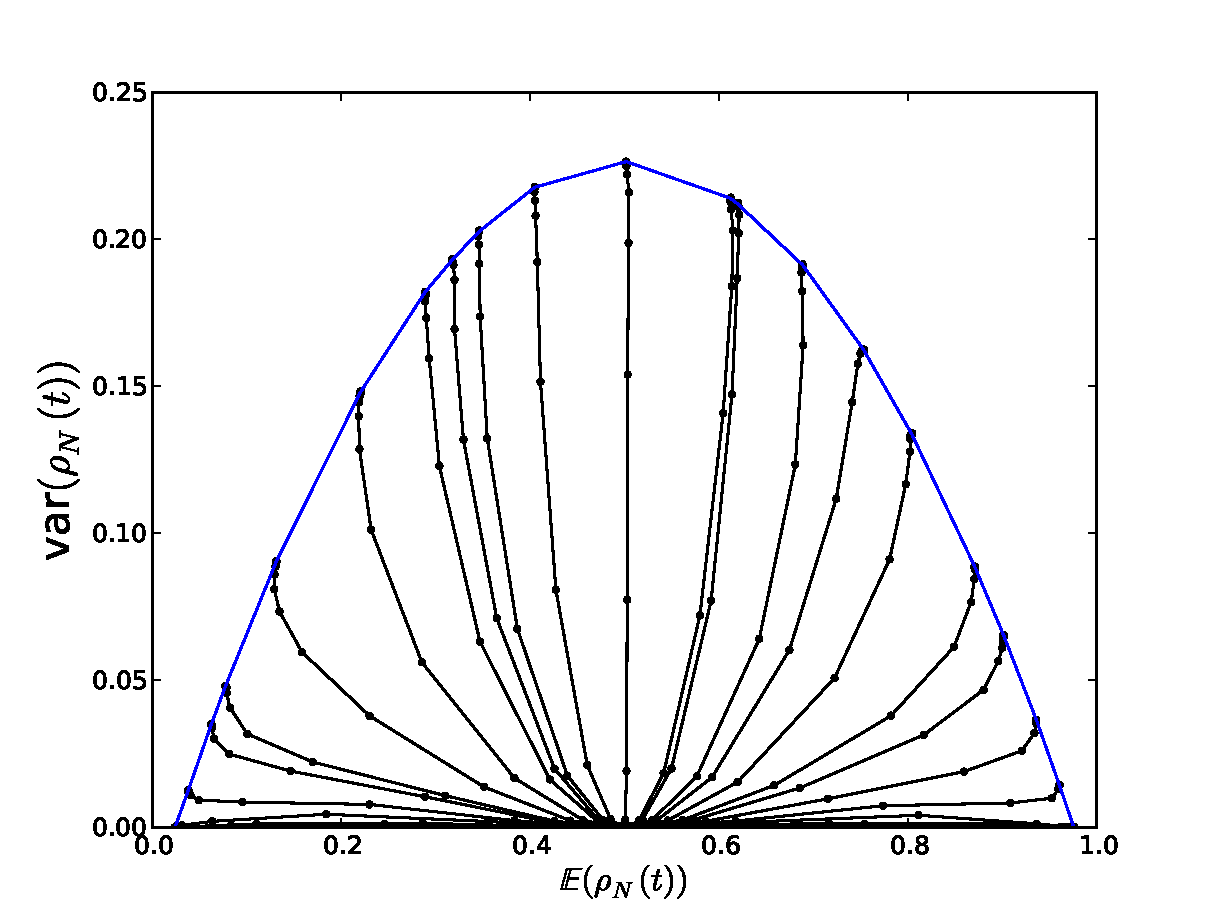
\includegraphics[width=0.9\textwidth]{sigma_variance_N1000_M500_fully_connected_20timesteps.pdf}
\caption{Expectation and variance of average states, starting from different initial conditions. For each trajectory, we initialise $M=500$ independent simulations for $N=1000$ agents and iterate the model until $t=20$.}
\label{fig:fig:variance_mean}
\end{figure}



\newpage{}


\bibliographystyle{plain}
\bibliography{biblio.bib}
\end{document}



